\documentclass[11pt]{beamer}

\usetheme{Singapore}

\definecolor{DarkRed}{rgb}{0.50,0,0}
\definecolor{DarkGreen}{rgb}{0,0.50,0}
\definecolor{DarkBlue}{rgb}{0,0,0.50}
\definecolor{Black}{rgb}{0,0,0}

\newcommand{\ttdr}[1]{{\tt{\color{DarkRed} #1}}}
\newcommand{\emdr}[1]{{\em{\color{DarkRed} #1}}}
\newcommand{\ttdg}[1]{{\tt{\color{DarkGreen} #1}}}
\newcommand{\emdg}[1]{{\em{\color{DarkGreen} #1}}}
\newcommand{\ttdb}[1]{{\tt{\color{DarkBlue} #1}}}
\newcommand{\emdb}[1]{{\em{\color{DarkBlue} #1}}}

\setbeamertemplate{frametitle}{
\begin{centering}
{\Large \textbf{\textmd{\insertframetitle}}}
\end{centering}
}

\setbeamertemplate{navigation symbols}{}

\setbeamertemplate{footline}{%
\begin{center}
{\color{DarkBlue}{\large 
\insertframenumber}
\hspace{240pt}

\includegraphics[height=20pt]{png/PDBP.png}}
\end{center}
}

\begin{document}

\begin{frame}
\vspace{25pt}
\begin{center}
\LARGE{
\vspace{10pt}
{\color{DarkGreen}{
PDBP}}} \\
\end{center}
\vspace{10pt}
\begin{center}
\LARGE{
{\color{DarkRed}{
Program Description Based Programming \\
Scala eXchange}}}
\end{center}
\vspace{10pt}
\begin{center}
\LARGE{
{\color{DarkBlue}{
Luc Duponcheel}}}
\end{center}
\vspace{10pt}
\begin{center}
\LARGE{
{\color{DarkGreen}{
\today}}}
\end{center}
\end{frame}

\begin{frame}[fragile]
\frametitle{\begin{center}Intro\end{center}}
\begin{itemize}
\item<2-> this talk is about
\begin{itemize}
\item<3-> a \ttdg{Dotty} \emdb{library} \ttdg{PDBP}
\item<4-> inspired by the \emdb{ function-level programming language} \ttdg{FP}
\end{itemize}
\end{itemize}
\end{frame}

\begin{frame}[fragile]
\frametitle{\begin{center}John Backus\end{center}}
\begin{center}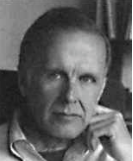
\includegraphics[height=60pt]{png/Backus.png}\end{center}
\begin{itemize}
\item<2-> ACM Turing Award Winner 1977
\item<3-> \emdb{Can programming be liberated from the Von Neumann style?}
\end{itemize}
\end{frame}

\begin{frame}[fragile]
\frametitle{\begin{center}What is this?\end{center}}
\begin{center}
\includegraphics[height=120pt]{png/PipeQuestion.png}\end{center}
\begin{itemize}
\item<2-> A \emdb{pipe}?
\item<3-> A painting \emdb{describing} a pipe?
\item<4-> A slide \emdb{describing} a painting describing a pipe?
\item<5-> \ldots
\end{itemize}
\end{frame}

\begin{frame}[fragile]
\frametitle{\begin{center}Ceci n'est pas une pipe\end{center}}
\begin{center}
\includegraphics[height=140pt]{png/Pipe.png}\end{center}
\begin{itemize}
\item<2-> It is a painting by Ren\'{e} Magritte \emdb{describing} a pipe
\end{itemize}
\end{frame}

\begin{frame}[fragile]
\frametitle{\begin{center}This is not a program\end{center}}
{\color{DarkGreen}	
\footnotesize{
\begin{verbatim}
  val program: BigInt >--> BigInt =
    `if`(isZero) {
      one
    } `else` {
      `let` {
        subtractOne >-->
          program
      } `in` {
        multiply
      }
    }
\end{verbatim}
}
}
\begin{center}
\begin{itemize}
\item<2-> It is \ttdg{Dotty} code \emdb{describing} a program
\item<3-> It is a \emdb{program description}
\item<4-> Can you think of a more meaningful name?
\end{itemize}
\end{center}
\end{frame}

\begin{frame}[fragile]
\frametitle{\begin{center}Program Description\end{center}}
\begin{itemize}
\item<2-> by abuse of notation we are simply going to write \emdb{program} instead of \emdb{program description}
\item<3-> we hope that this will not lead to any confusion
\end{itemize}
\end{frame}

\begin{frame}[fragile]
\frametitle{\begin{center}Type class \ttdg{Program}\end{center}}
{\color{DarkGreen}	
\footnotesize{
\begin{verbatim}
  trait Program[>-->[- _, + _]]
\end{verbatim}
}
}
\end{frame}

\begin{frame}[fragile]
\frametitle{\begin{center}\ttdg{factorial} program\end{center}}
{\color{DarkGreen}	
\footnotesize{
\begin{verbatim}
  val factorial: BigInt >--> BigInt =
    `if`(isZero) {
      one
    } `else` {
      `let` {
        subtractOne >-->
          factorial
      } `in` {
        multiply
      }
    }
\end{verbatim}
}
}
\begin{center}
\begin{itemize}
\item<2-> \ttdg{factorial} \emdb{definition} uses \\ the capabilities \emdb{declared} in \ttdg{Program}
\end{itemize}
\end{center}
\end{frame}

\begin{frame}[fragile]
\frametitle{\begin{center}\ttdg{factorial} implementations\end{center}}
{\color{DarkGreen}	
\footnotesize{
\begin{verbatim}
  val factorial: BigInt >--> BigInt =
    `if`(isZero) {
      one
    } `else` {
      `let` {
        subtractOne >-->
          factorial
      } `in` {
        multiply
      }
    }
\end{verbatim}
}
}
\begin{center}
\begin{itemize}
\item<2-> \ttdg{factorial} \emdb{implementations} depend on \\ \ttdg{implicit object}'s \emdb{defining} the capabilities of \ttdg{Program}
\end{itemize}
\end{center}
\end{frame}

\begin{frame}[fragile]
\frametitle{\begin{center}\ttdg{factorial} meanings\end{center}}
{\color{DarkGreen}	
\footnotesize{
\begin{verbatim}
  val factorial: BigInt >--> BigInt =
    `if`(isZero) {
      one
    } `else` {
      `let` {
        subtractOne >-->
          factorial
      } `in` {
        multiply
      }
    }
\end{verbatim}
}
}
\begin{center}
\begin{itemize}
\item<2-> \ttdg{factorial} \emdb{meanings} use \\ \emdb{natural transformations} transforming implementations
\end{itemize}
\end{center}
\end{frame}

\begin{frame}[fragile]
\frametitle{\begin{center}\ttdg{program}\end{center}}
{\color{DarkGreen}	
\begin{verbatim}
  val program: Z >--> Y
\end{verbatim}
}
\end{frame}

\begin{frame}[fragile]
\frametitle{\begin{center}\ttdg{Composition}\end{center}}
{\color{DarkGreen}	
\begin{verbatim}
  val `z>-->y`: Z >--> Y
  val `y>-->x`: Y >--> X

  val `z>-->x`: Z >--> X = `z>-->y >--> `y>-->x`
\end{verbatim}
}
\end{frame}

\begin{frame}[fragile]
\frametitle{\begin{center}\ttdg{program} \\ (design artifact)\end{center}}
{\color{DarkGreen}	
\begin{verbatim}
  
         --------------------------------
        |  ----------        ----------  |    
        | | Z >--> Y | >--> | Y >--> X | | 
        |  ----------        ----------  | 
         --------------------------------
                        ||
                        \/
                    ----------
                   | Z >--> X | 
                    ----------

\end{verbatim}
}
\end{frame}

\begin{frame}[fragile]
\frametitle{\begin{center}\ttdg{mainProgram}\end{center}}
{\color{DarkGreen}	
\begin{verbatim}
  val program: Unit >--> Unit
\end{verbatim}
}
\end{frame}

\begin{frame}[fragile]
\frametitle{\begin{center}\ttdg{mainProgram}\end{center}}
{\color{DarkGreen}	
\begin{verbatim}
  val producer: Unit >--> Z
  val program: Z >--> Y
  val consumer: Y >--> Unit

  val mainProgram: Unit >--> Unit =
    producer >--> program >--> consumer
\end{verbatim}
}
\end{frame}

\begin{frame}[fragile]
\frametitle{\begin{center}\ttdg{mainProgram} \\ (architectural artifact)\end{center}}
{\color{DarkGreen}	
\begin{verbatim}
  
    ------------------------------------------------
   |  ----------------    ----    ----------------  |     
   | | Unit >--> Unit |-| ???? |-| Unit >--> Unit | | 
   |  ----------------    ----    ----------------  | 
    ------------------------------------------------
                           ||
                           \/
                    ---------------- 
                   | Unit >--> Unit |
                    ----------------    

\end{verbatim}
}
\end{frame}

\begin{frame}[fragile]
\frametitle{\begin{center}\ttdg{FP} versus \ttdg{PDBP}\end{center}}
\begin{itemize}
\item<2-> \ttdg{FP} and \ttdg{PDBP} 
\begin{itemize}
\item<3-> promote \emdb{pointfree}, \emdb{composition} based, \emdb{functional programming}
\end{itemize}
\end{itemize}
\begin{itemize}
\item<4-> \ttdg{FP} is a \emdb{language} \\
\ttdg{PDBP} is a \emdb{library}
\begin{itemize}
\item<5-> \ttdg{FP} is \emdb{heterogeneous} \\ 
\ttdg{PDBP} is \emdb{homogeneous}
\item<6-> \ttdg{FP} \emdb{semantics} is \emdb{fixed} \\ 
\ttdg{PDBP} \emdb{semantics} is \emdb{not fixed}
\item<7-> \ttdg{FP} \emdb{capabilities} are \emdb{fixed} \\ 
\ttdg{PDBP} \emdb{capabilities} are \emdb{not fixed}
\item<8-> \ttdg{FP} \emdb{effects} are \emdb{impure} \\ 
\ttdg{PDBP} \emdb{effects} are \emdb{pure}
\end{itemize}
\end{itemize}
\end{frame}

\begin{frame}[fragile]
\frametitle{\begin{center}Homogeneous\end{center}}
\begin{itemize}
\item<2-> programs are objects
\begin{itemize}
\item<3-> programming using \ttdg{PDBP} is all about \\ \emdb{passing around programming capabilities}
\end{itemize}
\end{itemize}
\end{frame}

\begin{frame}[fragile]
\frametitle{\begin{center}Semantics\end{center}}
{\color{DarkGreen}	
\footnotesize{
\begin{verbatim}
  val factorial: BigInt >--> BigInt =
    `if`(isZero) {
      one
    } `else` {
      `let` {
        subtractOne >-->
          factorial
      } `in` {
        multiply
      }
    }
\end{verbatim}
}
}
\begin{itemize}
\item<2-> \emdb{production} 
\begin{itemize}
\item<3-> \emdb{recursion} using \emdb{stack} 
\item<4-> \emdb{recursion} using \emdb{heap}
\end{itemize}
\item<5-> \emdb{test}
\begin{itemize}
\item<6-> \ldots
\end{itemize}
\end{itemize}
\end{frame}

\begin{frame}[fragile]
\frametitle{\begin{center}Capabilities\end{center}}
\begin{itemize}
\item<2-> \emdb{manipulating state}
\item<3-> \emdb{handling failure}
\item<4-> \emdb{handling latency}
\item<5-> \emdb{handling control}
\item<6-> \emdb{\ldots}
\end{itemize}
\end{frame}

\begin{frame}[fragile]
\frametitle{\begin{center}Effects\end{center}}
\begin{itemize}
\item<2-> \emdb{reading} 
\item<3-> \emdb{writing}
\end{itemize}
\end{frame}

\begin{frame}[fragile]
\frametitle{\begin{center}Foundations\end{center}}
\begin{itemize}
\item<2-> \ttdg{trait Program[>-->[- \_, + \_]]} \\ corresponds to \emdb{arrows}
\item<3-> \ttdg{trait Computation[C[+ \_]]} \\ corresponds to \emdb{monads}
\end{itemize}
\end{frame}

\begin{frame}[fragile]
\frametitle{\begin{center}Arrows versus monads\end{center}}
\begin{itemize}
\item<2-> arrows generalize \emdb{functions}
\end{itemize}
\begin{itemize}
\item<3-> \emdb{composition} based, \emdb{pointfree} functional programming
\end{itemize}
\begin{itemize}
\item<4-> 
{\color{DarkGreen}
\footnotesize{
\begin{verbatim}
      val `z=>x`   = `z=>y` andThen `y=>x`
\end{verbatim}
}
}
\item<5-> 
{\color{DarkGreen}
\footnotesize{
\begin{verbatim}
      val `z>-->x` = `z>-->y` >-->  `y>-->z`
\end{verbatim}
}
}
\end{itemize}
\end{frame}


\begin{frame}[fragile]
\frametitle{\begin{center}Arrows versus monads\end{center}}
\begin{itemize}
\item<2-> monads generalize \emdb{expressions} 
\end{itemize}
\begin{itemize}
\item<3-> \emdb{binding} and \emdb{result} based, \emdb{pointful} functional programming
\end{itemize}
\begin{itemize}
\item<4-> 
{\color{DarkGreen}
\footnotesize{
\begin{verbatim}
      { val z = ez ; { val y = ey ; ex(z,y) } } 
\end{verbatim}
}
}
\item<5-> 
{\color{DarkGreen}
\footnotesize{
\begin{verbatim}
      mz bind { z => my bind { y => mx(z,y) } }
\end{verbatim}
}
}
\item<6-> 
{\color{DarkGreen}
\footnotesize{
\begin{verbatim}
      mz bind { z => my bind { y => result(ex(z,y)) } }
\end{verbatim}
}
}
\end{itemize}
\end{frame}

\begin{frame}[fragile]
\frametitle{\begin{center}Arrows versus monads (kleisli arrows)\end{center}}
\begin{itemize}
\item<2-> \ttdg{val function: Z => Y = { z => ey(x) }}
\begin{itemize}
\item<3-> expression is used to define function
\end{itemize}
\item<4-> \ttdg{val kleisliArrow: Z => M[Y] = { z => my(x) }}
\begin{itemize}
\item<5-> monad is used to define kleisli arrow
\end{itemize}
\end{itemize}
\end{frame}

\begin{frame}[fragile]
\frametitle{\begin{center}Arrows versus monads\end{center}}
\begin{itemize}
\item<2-> \emdb{arrows} can be programmed \emdb{pointful} (\emdb{arrow calculus})
\item<3-> \emdb{monads} can be programmed \emdb{pointfree} (\emdb{kleisli arrows}) 
\end{itemize}
\end{frame}

\begin{frame}[fragile]
\frametitle{\begin{center}Power of expressions\end{center}}
\begin{itemize}
\item<2-> \emdb{monads} are more \emdb{concrete} (less \emdb{abstract}) than \emdb{arrows}
\begin{itemize}
\item<3-> \emdb{monads allow more description liberty}
\item<4-> \emdb{monads impose more implementation constraints}
\end{itemize}
\item<5-> \emdb{Constraints Liberate, Liberties Constrain}
\end{itemize}
\end{frame}

\begin{frame}[fragile]
\frametitle{\begin{center}Elegance of use\end{center}}
\begin{itemize}
\item<2-> \emdb{pointfree} programming is sometimes considered to be \emdb{abstruse}
\item<3-> \ttdg{Dotty} comes to the rescue
\begin{itemize}
\item<4-> \ttdg{Dotty} is a \ttdg{Sca}lable \ttdg{la}nguage
\item<5-> \ttdg{Dotty} \emdb{library based} language extensions are \emdb{type safe}
\end{itemize}
\item<6-> \ttdg{PDBP} comes with a \emdb{program description DSL}
\end{itemize}
\end{frame}

\begin{frame}[fragile]
\frametitle{\begin{center}Program Description DSL\end{center}}
{\color{DarkGreen}	
\footnotesize{
\begin{verbatim}
  val factorial: BigInt >--> BigInt =
    `if`(isZero) {
      one
    } `else` {
      `let` {
        subtractOne >-->
          factorial
      } `in` {
        multiply
      }
    }
\end{verbatim}
}
}
\end{frame}

\begin{frame}[fragile]
\frametitle{\begin{center}Computation Description DSL\end{center}}
{\color{DarkGreen}	
\footnotesize{
\begin{verbatim}
  val factorial: BigInt => C[BigInt] = { z =>
    isZero(z) bind { b =>
      if (b) {
        one(z)
      } else {
        subtractOne(z) bind { y =>
          factorial(y) bind { x =>
            multiply((y, x))
          }
        }
      }
    }
  }
\end{verbatim}
}
}
\end{frame}

\begin{frame}[fragile]
\frametitle{\begin{center}Uh! Oh!\end{center}}
{\color{DarkGreen}	
\footnotesize{
\begin{verbatim}
  val factorial: BigInt => C[BigInt] = { z =>
    isZero(z) bind { b =>
      if (b) {
        one(z)
      } else {
        subtractOne(z) bind { y =>
          factorial(y) bind { x =>
            multiply((z, x))
          }
        }
      }
    }
  }
\end{verbatim}
}
}
\end{frame}
\begin{frame}[fragile]
\frametitle{\begin{center}\ttdg{PDBP}'s choice\end{center}}
\begin{itemize}
\item<2-> the \ttdg{PDBP} libary goes for
\begin{itemize}
\item<3-> \ttdg{private[pdbp]} \emdb{pointful monad API} \\
provides \emdb{power of expression} for \emdb{library} developers 
\item<4-> \ttdg{public} \emdb{pointfree arrow API} \\
provides \emdb{elegance of use} for \emdb{application} developers
\end{itemize}
\item<5->the \ttdg{PDBP} can live with
\begin{itemize}
\item<6-> corresponding implementation constraints
\end{itemize}
\end{itemize}
\end{frame}

\begin{frame}[fragile]
\frametitle{\begin{center}PDBP\end{center}}
{\color{DarkGreen}
\footnotesize{
\begin{verbatim}
  //       _______         __    __        _______
  //      / ___  /\       / /\  / /\      / ___  /\
  //     / /__/ / / _____/ / / / /_/__   / /__/ / /
  //    / _____/ / / ___  / / / ___  /\ /____  / /
  //   / /\____\/ / /__/ / / / /__/ / / \___/ / /
  //  /_/ /      /______/ / /______/ /     /_/ /
  //  \_\/       \______\/  \______\/      \_\/
  //                                           v1.0
  //  Program Description Based Programming Library
  //  author        Luc Duponcheel        2017-2018 
\end{verbatim}
}
}
\end{frame}

\begin{frame}[fragile]
\frametitle{\begin{center}\ttdg{PDBP} library design decisions\end{center}}
\begin{itemize}
\item<2-> \emdb{syntax} separated from \emdb{semantics}
\end{itemize}
\begin{itemize}
\item<3-> \emdb{syntax}
\begin{itemize}
\item<4-> \ttdg{trait}'s (\emdb{type classes}) \emdb{declare programming capabilities}
\item<5-> \emdb{program definitions} use them
\end{itemize}
\item<6-> \emdb{semantics}
\begin{itemize}
\item<7-> \ttdg{implicit object}'s \emdb{define programming capabilities} 
\item<8-> \emdb{program implementations} depend on them
\begin{itemize}
\item<9-> \emdb{implicitly}
\end{itemize}
\end{itemize}
\begin{itemize}
\item<10-> \ttdg{[implicit] object}'s \emdb{define natural transformations}
\item<11-> \emdb{program meanings} use them 
\begin{itemize}
\item<12-> \emdb{transforming program implementations}
\end{itemize}
\end{itemize}
\end{itemize}
\end{frame}

\begin{frame}[fragile]
\frametitle{\begin{center}\ttdg{PDBP} library design decisions\end{center}}
\begin{itemize}
\item<2-> programs are \emdb{defined} in \ttdg{class}'es \\ \emdb{declared} to \emdb{implicitly} have programming capabilities
\end{itemize}
\begin{itemize}
\item<3-> programs are \emdb{implemented} in \ttdg{object}'s \\ using \emdb{implicit dependency injection} by \ttdg{import}
\end{itemize}
\end{frame}

\begin{frame}[fragile]
\frametitle{\begin{center}\ttdg{Program} (cfr. \emdb{arrow})\end{center}}
{\color{DarkGreen}	
\footnotesize{
\begin{verbatim}
  trait Program[>-->[- _, + _]]
\end{verbatim}
}
}
\end{frame}

\begin{frame}[fragile]
\frametitle{\begin{center}\ttdg{Computation} (cfr. \emdb{monad})\end{center}}
{\color{DarkGreen}	
\footnotesize{
\begin{verbatim}
  trait Computation[C[+ _]]
\end{verbatim}
}
}
\end{frame}

\begin{frame}[fragile]
\frametitle{\begin{center}Liskov Substitution Principle\end{center}}
\begin{itemize}
\item<2-> \emdb{impose less}
\item<3-> \emdb{provide more}
\end{itemize}
\end{frame}

\begin{frame}[fragile]
\frametitle{\begin{center}Internet Robustness Principle\end{center}}
\begin{itemize}
\item<2-> \emdb{be liberal in what you receive}
\item<3-> \emdb{be generous in what you send}
\end{itemize}
\end{frame}

\begin{frame}[fragile]
\frametitle{\begin{center}\ttdg{PDBP} library details\end{center}}
\end{frame}

\begin{frame}[fragile]
\frametitle{\begin{center}\ttdg{Program}\end{center}}
{\color{DarkGreen}	
\footnotesize{
\begin{verbatim}
  trait Program[>-->[- _, + _]]
      extends Function[>-->] 
      with Composition[>-->] 
      with Construction[>-->] 
      with Condition[>-->]

      with Aggregation[>-->] 
\end{verbatim}
}
}
\begin{itemize}
\item<2-> \ttdg{trait}'s correspond to \ttdg{FP} \emdg{forms}
\end{itemize}
\end{frame}

\begin{frame}[fragile]
\frametitle{\begin{center}\ttdg{Function}\end{center}}
\begin{itemize}	
\item<2->
{\color{DarkGreen}	
\footnotesize{
\begin{verbatim}
      val `z>-->y` = function(`z=>y`) 
\end{verbatim}
}
}
\end{itemize}
\begin{itemize}
\item<3-> \emdb{pure functions} are \emdb{atomic programs}
\begin{itemize}	
\item<4-> up to you to define \emdb{granularity}
\end{itemize}
\end{itemize}
\end{frame}

\begin{frame}[fragile]
\frametitle{\begin{center}\ttdg{Composition}\end{center}}
\begin{itemize}	
\item<2->
{\color{DarkGreen}
\footnotesize{
\begin{verbatim}
      val `z>-->x` = `z>-->y` >--> `y>-->x`
\end{verbatim}
}
}
\end{itemize}
\end{frame}

\begin{frame}[fragile]
\frametitle{\begin{center}\ttdg{Construction}\end{center}}
\begin{itemize}	
\item<2->
{\color{DarkGreen}
\footnotesize{
\begin{verbatim}
      val `z>-->y&&x` = `z>-->y` & `z>-->x`
\end{verbatim}
}
}
\item<3->
{\color{DarkGreen}
\footnotesize{
\begin{verbatim}
      val `z&&y>-->x&&w` = `z>-->x` && `y>-->w`
\end{verbatim}
}
}
\end{itemize}
\begin{itemize}
\item<4->
{\color{DarkGreen}
\footnotesize{
\begin{verbatim}
      val `z>-->x` = 
        `let` `z>-->y` 
        `in` `z&&y>-->x`
\end{verbatim}
}
}
\end{itemize}
\end{frame}

\begin{frame}[fragile]
\frametitle{\begin{center}\ttdg{Condition}\end{center}}
\begin{itemize}	
\item<2->
{\color{DarkGreen}
\footnotesize{
\begin{verbatim}
      val `y||x>-->z` = `y>-->z` | `x>-->z`
\end{verbatim}
}
}
\item<3->
{\color{DarkGreen}
\footnotesize{
\begin{verbatim}
      val `x||w>-->z||y` = `x>-->z` || `w>-->y`
\end{verbatim}
}
}
\end{itemize}
\begin{itemize}
\item<4->
{\color{DarkGreen}
\footnotesize{
\begin{verbatim}
      val `y>-->z` = 
        `if`(`y>-->b`) `y>-t->z` 
        `else` `y>-f->z`
\end{verbatim}
}
}
\end{itemize}
\end{frame}

\begin{frame}[fragile]
\frametitle{\begin{center}\ttdg{Computation}\end{center}}
{\color{DarkGreen}	
\footnotesize{
\begin{verbatim}
  private[pdbp] trait Computation[C[+ _]]
      extends Resulting[C] 
      with Binding[C] 
      with Program[[-Z, +Y] => Z => C[Y]]

      with Lifting[C]

      with Sequencing[C]

\end{verbatim}
}
}
\end{frame}

\begin{frame}[fragile]
\frametitle{\begin{center}\ttdg{Resulting}\end{center}}
\begin{itemize}	
\item<2-> 
{\color{DarkGreen}	
\footnotesize{
\begin{verbatim}
  val cz = result(z)
\end{verbatim}
}
}
\end{itemize}
\end{frame}

\begin{frame}[fragile]
\frametitle{\begin{center}\ttdg{Binding}\end{center}}
\begin{itemize}	
\item<2-> 
{\color{DarkGreen}
\footnotesize{
\begin{verbatim}
  val cy = cz bind { z => `z=>cy`(y) }

\end{verbatim}
}
}
\item<3->
{\color{DarkGreen}
\footnotesize{
\begin{verbatim}
  val cy = cz bind { z => result(`z=>y`(y)) }
\end{verbatim}
}
}
\end{itemize}
\end{frame}

\begin{frame}[fragile]
\frametitle{\begin{center}\ttdg{Kleisli}\end{center}}
\begin{itemize}	
\item<2-> 
{\color{DarkGreen}
\footnotesize{
\begin{verbatim}
  type Kleisli[C[+ _]] = [-Z, + Y] => Z => C[Y]

\end{verbatim}
}
}
\item<3->
{\color{DarkGreen}
\footnotesize{
\begin{verbatim}
  private[pdbp] trait Computation[C[+ _]]
      extends Resulting[C] 
      with Binding[C] 
      with Program[Kleisli[C]]

      // ...
\end{verbatim}
}
}
\end{itemize}
\end{frame}

\begin{frame}[fragile]
\frametitle{\begin{center}\ttdg{factorial} Helper Functions\end{center}}
{\color{DarkGreen}	
\footnotesize{
\begin{verbatim}
  val isZeroFunction: BigInt => Boolean = { i =>
    i == 0
  }

  def oneFunction[Z]: Z => BigInt = { z =>
    1
  }

  val subtractOneFunction: BigInt => BigInt = { i =>
    i - 1
  }

  val multiplyFunction: (BigInt && BigInt) => BigInt = { (i, j) =>
    i * j
  }
\end{verbatim}
}
}
\end{frame}

\begin{frame}[fragile]
\frametitle{\begin{center}\ttdg{factorial} Helper Programs\end{center}}
{\color{DarkGreen}	
\footnotesize{
\begin{verbatim}
  val isZeroHelper: BigInt >--> Boolean =
    function(isZeroFunction)

  val subtractOneHelper: BigInt >--> BigInt =
    function(subtractOneFunction)

  val multiplyHelper: (BigInt && BigInt) >--> BigInt =
    function(multiplyFunction)

  def oneHelper[Z]: Z >--> BigInt =
    function(oneFunction)
\end{verbatim}
}
}
\end{frame}

\begin{frame}[fragile]
\frametitle{\begin{center}\ttdg{factorial} Atomic Programs\end{center}}
{\color{DarkGreen}	
\footnotesize{
\begin{verbatim}
  val isZero: BigInt >--> Boolean =
    isZeroHelper

  val subtractOne: BigInt >--> BigInt =
    subtractOneHelper

  val multiply: (BigInt && BigInt) >--> BigInt =
    multiplyHelper

  def one[Z]: Z >--> BigInt =
    oneHelper
\end{verbatim}
}
}
\end{frame}

\begin{frame}[fragile]
\frametitle{\begin{center}\ttdg{factorial} program\end{center}}
{\color{DarkGreen}	
\footnotesize{
\begin{verbatim}
  val factorial: BigInt >--> BigInt =
    `if`(isZero) {
      one
    } `else` {
      `let` {
        subtractOne >-->
          factorial
      } `in` {
        multiply
      }
    }
\end{verbatim}
}
}
\end{frame}

\begin{frame}[fragile]
\frametitle{\begin{center}\ttdg{mainFactorial}\end{center}}
{\color{DarkGreen}	
\footnotesize{
\begin{verbatim}
  val producer: Unit >--> BigInt

  val consumer: BigInt >--> Unit

  lazy val mainFactorial: Unit >--> Unit =
    producer >-->
      factorial >-->
      consumer
\end{verbatim}
}
}
\end{frame}

\begin{frame}[fragile]
\frametitle{\begin{center}\ttdg{activeTypes}\end{center}}
{\color{DarkGreen}	
\footnotesize{
\begin{verbatim}
  object activeTypes {

    type Active[+Z] = Z

    type `=>A` = Kleisli[Active]

  }
\end{verbatim}
}
}
\end{frame}

\begin{frame}[fragile]
\frametitle{\begin{center}\ttdg{activeProgram}\end{center}}
{\color{DarkGreen}	
\footnotesize{
\begin{verbatim}
  implicit object activeProgram
      extends Computation[Active]
      with Program[`=>A`] {

    override private[pdbp] def result[Z]: Z => Active[Z] = 
      `z=>az`

    override private[pdbp] def bind[Z, Y](
        az: Active[Z],
        `z=>ay`: => (Z => Active[Y])): Active[Y] = 
      `z=>ay`(az)  

  }
\end{verbatim}
}
}
\end{frame}

\begin{frame}[fragile]
\frametitle{\begin{center}\ttdg{activeMeaningOfActive}\end{center}}
{\color{DarkGreen}	
\footnotesize{
\begin{verbatim}
  implicit object activeMeaningOfActive
      extends MeaningOfActive[Active]()
      with ComputationMeaning[Active, Active]()
      with ProgramMeaning[`=>A`, `=>A`]()    
\end{verbatim}
}
}
\end{frame}

\begin{frame}[fragile]
\frametitle{\begin{center}\ttdg{FactorialMain}\end{center}}
{\color{DarkGreen}	
\footnotesize{
\begin{verbatim}
import ... activeTypes._

import ... implicits.activeProgram

import ... MainFactorial
\end{verbatim}
}
}
\end{frame}

\begin{frame}[fragile]
\frametitle{\begin{center}Effectful producer and consumer\end{center}}
{\color{DarkGreen}	
\footnotesize{
\begin{verbatim}
  private def effectfulReadIntFromConsoleWithMessage(
      message: String): Unit >--> BigInt =
    function(effectfulReadIntFromConsoleFunction(message))

  private def effectfulWriteLineToConsoleWithMessage[Y](
      message: String): Y >--> Unit =
    function[Y, Unit](effectfulWriteLineToConsoleFunction(message))

  val effectfulReadIntFromConsole: Unit >--> BigInt =
    effectfulReadIntFromConsoleWithMessage("please type an integer")

  val effectfulWriteFactorialOfIntToConsole: BigInt >--> Unit =
    effectfulWriteLineToConsoleWithMessage(
      "the factorial value of the integer is")
\end{verbatim}
}
}
\end{frame}

\begin{frame}[fragile]
\frametitle{\begin{center}\ttdg{FactorialMain}\end{center}}
{\color{DarkGreen}	
\footnotesize{
\begin{verbatim}
object FactorialMain extends MainFactorial[`=>A`]() {

  // ... effectful utilities

  override val producer = 
    effectfulReadIntFromConsole

  override val consumer = 
    effectfulWriteFactorialOfIntToConsole

}
\end{verbatim}
}
}
\end{frame}

\begin{frame}[fragile]
\frametitle{\begin{center}\ttdg{FactorialMain}\end{center}}
{\color{DarkGreen}	
\footnotesize{
\begin{verbatim}
object FactorialMain extends MainFactorial[`=>A`]() {

  def main(args: Array[String]): Unit = {

    import ... activeMeaningOfActive.meaning

    meaning(mainFactorial)(())

  }

}
\end{verbatim}
}
}
\end{frame}

\begin{frame}[fragile]
\frametitle{\begin{center}Problems and Solutions\end{center}}
\begin{itemize}
\item<2-> Problem: \\ the \ttdg{factorial} semantics above \emdb{is not stack safe}
\item<3-> Solution: \\ \ttdg{FreeTransformation} and \ttdg{FreeTransformedMeaning}
\end{itemize}
\begin{itemize}
\item<4-> Problem: \\ \ttdg{producer} and \ttdg{consumer} above \emdb{execute effects}
\item<5-> Solution: \\ \ttdg{read} and \ttdg{write} \emdb{describe effects}
\end{itemize}
\end{frame}

\begin{frame}[fragile]
\frametitle{\begin{center}\ttdg{ComputationTransformation}\end{center}}
{\color{DarkGreen}	
\footnotesize{
\begin{verbatim}
private[pdbp] trait ComputationTransformation[
    FC[+ _]: Computation, 
    T[+ _]] 
    extends Computation[T]
    with Program[Kleisli[T]] {

  private[pdbp] val transform: FC `-U->` T

}
\end{verbatim}
}
}
\begin{itemize}
\item<2-> \emdb{computation transformations} transform \\ \emdb{computations} \ttdg{FC} (and corresponding \emdb{kleisli programs}) to \\ \emdb{computations} \ttdg{T } (and corresponding \emdb{kleisli programs}) 
\end{itemize}
\end{frame}

\begin{frame}[fragile]
\frametitle{\begin{center}\ttdg{ProgramMeaning}\end{center}}
{\color{DarkGreen}	
\footnotesize{
\begin{verbatim}
  trait ProgramMeaning[
    `>-FP->`[- _, + _]: Program, 
    `>-T->`[- _, + _]] {

    private[pdbp] lazy val binaryTransformation: 
        `>-FP->` `-B->` `>-T->`

    lazy val meaning: `>-FP->` `-B->` `>-T->` = 
      binaryTransformation

  }
\end{verbatim}
}
}
\end{frame}

\begin{frame}[fragile]
\frametitle{\begin{center}\ttdg{ComputationMeaning}\end{center}}
{\color{DarkGreen}	
\footnotesize{
\begin{verbatim}
  private[pdbp] trait ComputationMeaning[
    FC[+ _]: Computation, T[+ _]]
      extends ProgramMeaning[Kleisli[FC], Kleisli[T]] {

    private[pdbp] val unaryTransformation: FC `-U->` T

    // ...

  }
\end{verbatim}
}
}
\begin{itemize}
\item<2-> \emdb{computation meanings} are \\  \emdb{program meanings} for corresponding kleisli programs
\end{itemize}
\end{frame}

\begin{frame}[fragile]
\frametitle{\begin{center}\ttdg{FreeTransformed}\end{center}}
{\color{DarkGreen}	
\footnotesize{
\begin{verbatim}
  sealed trait Free[C[+ _], +Z]

  final case class Transform[C[+ _], +Z]
    (cz: C[Z]) extends Free[C, Z]
  final case class Result[C[+ _], +Z]
    (z: Z) extends Free[C, Z]
  final case class Bind[C[+ _], -Z, ZZ <: Z, +Y]
    (fczz: Free[C, ZZ], `z=>fcy`: Z => Free[C, Y])
      extends Free[C, Y]

  type FreeTransformed[C[+ _]] = [+Z] => Free[C, Z]
\end{verbatim}
}
}
\end{frame}

\begin{frame}[fragile]
\frametitle{\begin{center}\ttdg{FreeTransformation}\end{center}}
{\color{DarkGreen}	
\footnotesize{
\begin{verbatim}
  private[pdbp] 
    trait FreeTransformation[FC[+ _]: Computation]
        extends ComputationTransformation[
          FC, 
          FreeTransformed[FC]] {

    // unfold


    // transform => Transform

    // result => Result
    // bind => Bind

  }
\end{verbatim}
}
}
\end{frame}

\begin{frame}[fragile]
\frametitle{\begin{center}\ttdg{activeFreeTypes}\end{center}}
{\color{DarkGreen}	
\footnotesize{
\begin{verbatim}
  object activeFreeTypes {

    type ActiveFree = FreeTransformed[Active]

    type `=>AF` = Kleisli[ActiveFree]

  }
\end{verbatim}
}
}
\end{frame}

\begin{frame}[fragile]
\frametitle{\begin{center}\ttdg{activeFreeProgram}\end{center}}
{\color{DarkGreen}	
\footnotesize{
\begin{verbatim}
  import ... implicits.activeProgram

  implicit object activeFreeProgram
      extends Computation[ActiveFree]
      with Program[`=>AF`]

      with FreeTransformation[Active]()
      with ComputationTransformation[Active, ActiveFree]()
\end{verbatim}
}
}
\end{frame}

\begin{frame}[fragile]
\frametitle{\begin{center}\ttdg{FreeTransformedMeaning}\end{center}}
{\color{DarkGreen}	
\footnotesize{
\begin{verbatim}
  private[pdbp] trait FreeTransformedMeaning[
    FC[+ _]: Computation, T[+ _]](
    implicit toBeTransformedMeaning:
      ComputationMeaning[FC, T])
      extends ComputationMeaning[FreeTransformed[FC], T] {

    // fold (tail recursive)


    // Transform(fcz) => fcz

    // Result(z) => result(z)
    // Bind(Result(y), y2ftfcz) => fold(y2ftfcz(y))
    // Bind(Bind(fcx, x2ftfcy), y2ftfcz) => 
    //   fold(Bind(fcx, Bind(x2ftfcy, y2ftfcz)))

  }       
\end{verbatim}
}
}
\end{frame}

\begin{frame}[fragile]
\frametitle{\begin{center}\ttdg{activeMeaningOfActiveFree}\end{center}}
{\color{DarkGreen}	
\footnotesize{
\begin{verbatim}
  import ... activeMeaningOfActive

  implicit object activeMeaningOfActiveFree
      extends FreeTransformedMeaning[Active, Active]()
      with ComputationMeaning[ActiveFree, Active]()

      with ProgramMeaning[`=>AF`, `=>A`]()    
\end{verbatim}
}
}
\end{frame}

\begin{frame}[fragile]
\frametitle{\begin{center}\ttdg{FactorialMain}\end{center}}
{\color{DarkGreen}	
\footnotesize{
\begin{verbatim}
import ... activeFreeTypes._

import ... implicits.activeFreeProgram

import ... MainFactorial
\end{verbatim}
}
}
\end{frame}

\begin{frame}[fragile]
\frametitle{\begin{center}\ttdg{FactorialMain}\end{center}}
{\color{DarkGreen}	
\footnotesize{
\begin{verbatim}
object FactorialMain extends MainFactorial[`=>AF`]() {

  // ... effectful utilities

  override val producer = effectfulReadIntFromConsole

  override val consumer = effectfulWriteFactorialOfIntToConsole

}
\end{verbatim}
}
}
\end{frame}

\begin{frame}[fragile]
\frametitle{\begin{center}\ttdg{FactorialMain}\end{center}}
{\color{DarkGreen}	
\footnotesize{
\begin{verbatim}
object FactorialMain extends MainFactorial[`=>AF`]() {

  def main(args: Array[String]): Unit = {

    import ... activeMeaningOfActiveFree.meaning

    meaning(mainFactorial)(())

  }

}
\end{verbatim}
}
}
\end{frame}

\begin{frame}[fragile]
\frametitle{\begin{center}\ttdg{Reading}\end{center}}
{\color{DarkGreen}	
\footnotesize{
\begin{verbatim}
  trait Reading[R, >-->[- _, + _]] {
    

    private[pdbp] def `u>-->r`: Unit >--> R 






  }
\end{verbatim}
}
}
\end{frame}

\begin{frame}[fragile]
\frametitle{\begin{center}\ttdg{Reading}\end{center}}
{\color{DarkGreen}	
\footnotesize{
\begin{verbatim}
  trait Reading[R, >-->[- _, + _]] {
    this: Function[>-->] & Composition[>-->] =>

    private[pdbp] def `u>-->r`: Unit >--> R =
      read[Unit]




    def read[Z]: Z >--> R

  }
\end{verbatim}
}
}
\end{frame}

\begin{frame}[fragile]
\frametitle{\begin{center}\ttdg{Reading}\end{center}}
{\color{DarkGreen}	
\footnotesize{
\begin{verbatim}
  trait Reading[R, >-->[- _, + _]] {
    this: Function[>-->] & Composition[>-->] =>

    private[pdbp] def `u>-->r`: Unit >--> R = 
      read[Unit]

    private[pdbp] def `z>-->r`[Z]: Z >--> R =
      compose(`z>-->u`, `u>-->r`)

    def read[Z]: Z >--> R = `z>-->r`

  }
\end{verbatim}
}
}
\end{frame}

\begin{frame}[fragile]
\frametitle{\begin{center}implicit function type\end{center}}
{\color{DarkGreen}	
\footnotesize{
\begin{verbatim}
  type `I=>`[-X, +Y] = implicit X => Y
\end{verbatim}
}
}
\begin{itemize}
\item<2-> \emdb{reduces boilerplate} of \emdb{reading} code
\item<3-> \emdb{optimizes performance} of \emdb{reading} code
\end{itemize}
\end{frame}

\begin{frame}[fragile]
\frametitle{\begin{center}\ttdg{ReadingTransformed}\end{center}}
{\color{DarkGreen}	
\footnotesize{
\begin{verbatim}
  type ReadingTransformed[R, C[+ _]] = 
    [+Z] => R `I=>` C[Z]
\end{verbatim}
}
}
\end{frame}

\begin{frame}[fragile]
\frametitle{\begin{center}\ttdg{ReadingTransformation}\end{center}}
{\color{DarkGreen}	
\footnotesize{
\begin{verbatim}
  private[pdbp] trait ReadingTransformation[
    R, FC[+ _]: Computation]
      extends ComputationTransformation[
        FC, 
        ReadingTransformed[R, FC]]

      with Reading[
        R, 
        Kleisli[ReadingTransformed[R, FC]]] {

    // ...

  }      
\end{verbatim}
}
}
\end{frame}

\begin{frame}[fragile]
\frametitle{\begin{center}\ttdg{activeReadingTypes}\end{center}}
{\color{DarkGreen}	
\footnotesize{
\begin{verbatim}
  object activeReadingTypes {

    type ActiveReading[R] = ReadingTransformed[R, Active]

    type `=>AR`[R] = Kleisli[ActiveReading[R]]

  }
\end{verbatim}
}
}
\end{frame}

\begin{frame}[fragile]
\frametitle{\begin{center}\ttdg{ActiveReadingProgram}\end{center}}
{\color{DarkGreen}	
\footnotesize{
\begin{verbatim}
private[pdbp] trait ActiveReadingProgram[R]
    extends Computation[ActiveReading[R]]
    with Program[`=>AR`[R]]
    with Reading[R, `=>AR`[R]]

    with ComputationTransformation[Active, ActiveReading[R]]
    with ReadingTransformation[R, Active]
\end{verbatim}
}
}
\end{frame}

\begin{frame}[fragile]
\frametitle{\begin{center}\ttdg{activeIntReadingProgram}\end{center}}
{\color{DarkGreen}	
\footnotesize{
\begin{verbatim}
  import  ... implicits.activeProgram

  implicit object activeIntReadingProgram
      extends ActiveReadingProgram[BigInt]()
      with Computation[ActiveReading[BigInt]]()
      with Program[`=>AR`[BigInt]]()
      with Reading[BigInt, `=>AR`[BigInt]]()  

      with ReadingTransformation[BigInt, Active]()
      with ComputationTransformation[Active, ActiveReading[BigInt]]()
\end{verbatim}
}
}
\end{frame}

\begin{frame}[fragile]
\frametitle{\begin{center}\ttdg{ReadingTransformedMeaning}\end{center}}
{\color{DarkGreen}	
\footnotesize{
\begin{verbatim}
private[pdbp] trait ReadingTransformedMeaning[
      R, 
      FC[+ _]: Computation, 
      T[+ _]](
    implicit toBeTransformedMeaning:
      ComputationMeaning[FC, T])
    extends ComputationMeaning[
        ReadingTransformed[R, FC],
        ReadingTransformed[R, T]]
\end{verbatim}
}
}
\end{frame}

\begin{frame}[fragile]
\frametitle{\begin{center}\ttdg{activeIntReadingMeaningOfActiveIntReading}\end{center}}
{\color{DarkGreen}	
\footnotesize{
\begin{verbatim}
  import ... activeIntReadingProgram

  implicit object activeIntReadingMeaningOfActiveIntReading
      extends ReadingTransformedMeaning[
        BigInt, Active, Active]()
      with ComputationMeaning[
        ActiveReading[BigInt], 
        ActiveReading[BigInt]]()

      with ProgramMeaning[
        `=>AR`[BigInt], 
        `=>AR`[BigInt]]()
\end{verbatim}
}
}
\end{frame}

\begin{frame}[fragile]
\frametitle{\begin{center}\ttdg{FactorialOfIntReadMain}\end{center}}
{\color{DarkGreen}	
\footnotesize{
\begin{verbatim}
import ... activeReadingTypes._

import ... implicits.activeIntReadingProgram

import ... MainFactorial
\end{verbatim}
}
}
\end{frame}

\begin{frame}[fragile]
\frametitle{\begin{center}\ttdg{readIntFromConsoleEffect}\end{center}}
{\color{DarkGreen}	
\footnotesize{
\begin{verbatim}

  private def readIntFromConsoleEffectWithMessage(
    message: String): BigInt =
    effectfulReadIntFromConsoleFunction(message)(())

  implicit val readIntFromConsoleEffect: BigInt =
    readIntFromConsoleEffectWithMessage(
      "please type an integer to read")

\end{verbatim}
}
}
\end{frame}

\begin{frame}[fragile]
\frametitle{\begin{center}\ttdg{FactorialOfIntReadMain}\end{center}}
{\color{DarkGreen}	
\footnotesize{
\begin{verbatim}
object FactorialOfIntReadMain
    extends MainFactorial[`=>AR`[BigInt]]() {

  // ... effectful utilities

  import ... readIntFromConsoleEffect

  override val producer = 
    activeIntReadingProgram.read

  override val consumer = 
    effectfulWriteFactorialOfIntReadToConsole

}
\end{verbatim}
}
}
\end{frame}

\begin{frame}[fragile]
\frametitle{\begin{center}\ttdg{FactorialOfIntReadMain}\end{center}}
{\color{DarkGreen}	
\footnotesize{
\begin{verbatim}
object FactorialOfIntReadMain
    extends MainFactorial[`=>AR`[BigInt]]() {

  def main(args: Array[String]): Unit = {

    ... activeIntReadingMeaningOfActiveIntReading.meaning

    meaning(mainFactorial)(())

  }

}
\end{verbatim}
}
}
\end{frame}

\begin{frame}[fragile]
\frametitle{\begin{center}\ttdg{factorialMultipliedByIntRead}\end{center}}
{\color{DarkGreen}	
\footnotesize{
\begin{verbatim}
  val factorialMultipliedByIntRead: BigInt >--> BigInt =
      (factorial & read) >--> multiply 
\end{verbatim}
}
}
\end{frame}

\begin{frame}[fragile]
\frametitle{\begin{center}\ttdg{MainFactorialMultipliedByIntRead}\end{center}}
{\color{DarkGreen}	
\footnotesize{
\begin{verbatim}
trait MainFactorialMultipliedByIntRead[
    >-->[- _, + _]: Program
                  : [>-->[- _, + _]] => Reading[BigInt, >-->]] {

  // ...

  lazy val mainFactorialMultipliedByIntRead: Unit >--> Unit =
    producer >-->
      factorialMultipliedByIntRead >-->
      consumer

}
\end{verbatim}
}
}
\end{frame}


\begin{frame}[fragile]
\frametitle{\begin{center}\ttdg{FactorialMultipliedByIntReadMain}\end{center}}
{\color{DarkGreen}	
\footnotesize{
\begin{verbatim}
object FactorialMultipliedByIntReadMain
    extends MainFactorialMultipliedByIntRead[`=>AR`[BigInt]]() {

  // effectful utilities

  override val producer =
    effectfulReadIntFromConsole

  override val consumer =
    effectfulWriteFactorialOfIntMultipliedByIntReadToConsole

}
\end{verbatim}
}
}
\end{frame}

\begin{frame}[fragile]
\frametitle{\begin{center}\ttdg{FactorialMultipliedByIntReadMain}\end{center}}
{\color{DarkGreen}	
\footnotesize{
\begin{verbatim}
object FactorialMultipliedByIntReadMain
    extends MainFactorialMultipliedByIntRead[`=>AR`[BigInt]]() {

  def main(args: Array[String]): Unit = {

    import ... readIntFromConsoleEffect

    import ... activeIntReadingMeaningOfActiveIntReading.meaning

    meaning(mainFactorialMultipliedByIntRead)(())

  }

}
\end{verbatim}
}
}
\end{frame}

\begin{frame}[fragile]
\frametitle{\begin{center}\ttdg{Writing}\end{center}}
{\color{DarkGreen}	
\footnotesize{
\begin{verbatim}
  trait Writing[W: Writable, >-->[- _, + _]] {
    

    private[pdbp] val `w>-->u`: W >--> Unit  









  }
\end{verbatim}
}
}
\end{frame}

\begin{frame}[fragile]
\frametitle{\begin{center}\ttdg{Writing}\end{center}}
{\color{DarkGreen}	
\footnotesize{
\begin{verbatim}
  trait Writing[W: Writable, >-->[- _, + _]] {
    this: Function[>-->] & Composition[>-->] =>

    private[pdbp] val `w>-->u`: W >--> Unit =
      write(identity)





    def write[Z]:                Z >--> Unit
       

  }
\end{verbatim}
}
}
\end{frame}

\begin{frame}[fragile]
\frametitle{\begin{center}\ttdg{Writing}\end{center}}
{\color{DarkGreen}	
\footnotesize{
\begin{verbatim}
  trait Writing[W: Writable, >-->[- _, + _]] {
    this: Function[>-->] & Composition[>-->] =>

    private[pdbp] val `w>-->u`: W >--> Unit = 
      write(identity)





    def write[Z]: (Z => W) `I=>` Z >--> Unit


  }
\end{verbatim}
}
}
\end{frame}

\begin{frame}[fragile]
\frametitle{\begin{center}\ttdg{Writing}\end{center}}
{\color{DarkGreen}	
\footnotesize{
\begin{verbatim}
  trait Writing[W: Writable, >-->[- _, + _]] {
    this: Function[>-->] & Composition[>-->] =>

    private[pdbp] val `w>-->u`: W >--> Unit = 
      write(identity)

    private[pdbp] def `z>-w->u`[Z]: 
        (Z => W) `I=>` Z >--> Unit =
      compose(function(implicitly), `w>-->u`)

    def write[Z]: (Z => W) `I=>` Z >--> Unit =
      `z>-w->u`

  }
\end{verbatim}
}
}
\end{frame}

\begin{frame}[fragile]
\frametitle{\begin{center}\ttdg{Writing}\end{center}}
{\color{DarkGreen}	
\footnotesize{
\begin{verbatim}
  def writingUsing[Z, Y,  ](
                                  ): 
      (Z >--> Y) => (               Z >--> Y)













      
\end{verbatim}
}
}
\end{frame}

\begin{frame}[fragile]
\frametitle{\begin{center}\ttdg{Writing}\end{center}}
{\color{DarkGreen}	
\footnotesize{
\begin{verbatim}
  def writingUsing[Z, Y, X](
      `(z&&y)=>x`: ((Z && Y) => X)): 
      (Z >--> Y) => (               Z >--> Y)













      
\end{verbatim}
}
}
\end{frame}

\begin{frame}[fragile]
\frametitle{\begin{center}\ttdg{Writing}\end{center}}
{\color{DarkGreen}	
\footnotesize{
\begin{verbatim}
  def writingUsing[Z, Y, X](
      `(z&&y)=>x`: ((Z && Y) => X)): 
      (Z >--> Y) => ((X => W) `I=>` Z >--> Y)













      
\end{verbatim}
}
}
\end{frame}

\begin{frame}[fragile]
\frametitle{\begin{center}\ttdg{Writing}\end{center}}
{\color{DarkGreen}	
\footnotesize{
\begin{verbatim}
  def writingUsing[Z, Y, X](
      `(z&&y)=>x`: ((Z && Y) => X)): 
      (Z >--> Y) => ((X => W) `I=>` Z >--> Y) = { `z>-->y` =>
      val `(z&&y)>-->x` = function(`(z&&y)=>x`)
      val `z>-->(x&&y)` =
        `let` {
          `z>-->y`
        } `in` {
          `let` {
            `(z&&y)>-->x`
          } `in` {
            `(z&&y&&x)>-->(x&&y)`
          }
        }
      compose(compose(`z>-->(x&&y)`, left(write), 
        `(u&&y)>-->y`)
  }          
\end{verbatim}
}
}
\end{frame}

\begin{frame}[fragile]
\frametitle{\begin{center}\ttdg{Writable} (cfr. \emdb{monoid})\end{center}}
{\color{DarkGreen}	
\footnotesize{
\begin{verbatim}
  private[pdbp] trait Writable[W]
      extends Startable[W]
      with Appendable[W]
\end{verbatim}
}
}
\end{frame}

\begin{frame}[fragile]
\frametitle{\begin{center}\ttdg{Startable}\end{center}}
{\color{DarkGreen}	
\footnotesize{
\begin{verbatim}
  private[pdbp] trait Startable[W] {

    private[pdbp] val start: W

  }
\end{verbatim}
}
}
\end{frame}

\begin{frame}[fragile]
\frametitle{\begin{center}\ttdg{Appendable}\end{center}}
{\color{DarkGreen}	
\footnotesize{
\begin{verbatim}
  private[pdbp] trait Appendable[W] {

    private[pdbp] val append: W && W => W

  }
\end{verbatim}
}
}
\end{frame}

\begin{frame}[fragile]
\frametitle{\begin{center}\ttdg{WritingTransformed}\end{center}}
{\color{DarkGreen}	
\footnotesize{
\begin{verbatim}
  type WritingTransformed[W, FC[+ _]] = 
    [+Z] => FC[W && Z]
\end{verbatim}
}
}
\end{frame}

\begin{frame}[fragile]
\frametitle{\begin{center}\ttdg{WritingTransformation}\end{center}}
{\color{DarkGreen}	
\footnotesize{
\begin{verbatim}
  private[pdbp] trait WritingTransformation[
    W: Writable, FC[+ _]: Computation]
      extends ComputationTransformation[
        FC, WritingTransformed[W, FC]]

      with Writing[
        W, 
        Kleisli[WritingTransformed[W, FC]]] {

    // ...

  }      
\end{verbatim}
}
}
\end{frame}

\begin{frame}[fragile]
\frametitle{\begin{center}\ttdg{ToConsole}\end{center}}
{\color{DarkGreen}	
\footnotesize{
\begin{verbatim}
  case class ToConsole(effect: Effect)

  type Effect = Unit => Unit
\end{verbatim}
}
}
\end{frame}

\begin{frame}[fragile]
\frametitle{\begin{center}\ttdg{toConsoleWritable}\end{center}}
{\color{DarkGreen}	
\footnotesize{
\begin{verbatim}
  implicit object toConsoleWritable extends Writable[ToConsole] {

    override private[pdbp] val start: ToConsole =
      ToConsole { _ =>
        ()
      }

    override private[pdbp] val append: 
        ToConsole && ToConsole => ToConsole = {
      (tc1, tc2) =>
        ToConsole { _ =>
          { tc1.effect(()); tc2.effect(()) }
        }
    }

  }
\end{verbatim}
}
}
\end{frame}

\begin{frame}[fragile]
\frametitle{\begin{center}\ttdg{WritingToConsoleTransformedMeaning}\end{center}}
{\color{DarkGreen}	
\footnotesize{
\begin{verbatim}
  private[pdbp] trait WritingToConsoleTransformedMeaning[
      FC[+ _]: Computation,
      T[+ _]]
      (implicit toBeTransformedMeaning: 
        ComputationMeaning[FC, T])
      extends ComputationMeaning[
        WritingTransformed[ToConsole, FC], 
          T] {

    // executes console effect

}       
\end{verbatim}
}
}
\end{frame}

\begin{frame}[fragile]
\frametitle{\begin{center}\ttdg{infoUtils}\end{center}}
{\color{DarkGreen}	
\footnotesize{
\begin{verbatim}
  def infoFunction[Z, Y](string: String): Z && Y => String = {
    case (z, y) =>
      s"INFO -- $currentCalendarInMilliseconds -- $string($z) => $y"
  }

  def info[
      W: Writable, Z, Y,  
      >-->[- _, + _]: [>-->[- _, + _]] => Writing[W, >-->]]
      (string: String): 
      (Z >--> Y) => ((String => W) `I=>` Z >--> Y) = {
    val implicitWriting = implicitly[Writing[W, >-->]]
    implicitWriting.writingUsing(infoFunction(string))
  }
\end{verbatim}
}
}
\end{frame}

\begin{frame}[fragile]
\frametitle{\begin{center}\ttdg{WritingAtomicPrograms}\end{center}}
{\color{DarkGreen}	
\footnotesize{
\begin{verbatim}
  val isZero: (String => W) `I=>` BigInt >--> Boolean =
    info("isZero") { isZeroHelper }

  val subtractOne: (String => W) `I=>` BigInt >--> BigInt =
    info("subtractOne") { subtractOneHelper }

  val multiply: (String => W) `I=>` (BigInt && BigInt) >--> BigInt =
    info("multiply") { multiplyHelper }

  def one[Z]: (String => W) `I=>` Z >--> BigInt =
    info("one") { oneHelper }
\end{verbatim}
}
}
\end{frame}

\begin{frame}[fragile]
\frametitle{\begin{center}\ttdg{WritingFactorial}\end{center}}
{\color{DarkGreen}	
\footnotesize{
\begin{verbatim}
  val factorial: (String => W) `I=>` BigInt >--> BigInt =
    info("factorial") {
      `if`(isZero) {
        one
      } `else` {
        `let` {
          subtractOne >-->
            factorial
        } `in` {
          multiply
        }
      }
    }
\end{verbatim}
}
}
\end{frame}

\begin{frame}[fragile]
\frametitle{\begin{center}\ttdg{MainWritingFactorial}\end{center}}
{\color{DarkGreen}	
\footnotesize{
\begin{verbatim}
trait MainWritingFactorial[
    W: Writable,
    >-->[- _, + _]: Program
                  : [>-->[- _, + _]] => Writing[W, >-->]] {

  // ...

  lazy val mainWritingFactorial: 
      (String => W) `I=>` Unit >--> Unit = {
    producer >-->
      writingFactorial >-->
      consumer
  }

}
\end{verbatim}
}
}
\end{frame}

\begin{frame}[fragile]
\frametitle{\begin{center}\ttdg{activeWritingToConsoleProgram}\end{center}}
{\color{DarkGreen}	
\footnotesize{
\begin{verbatim}
  import ... toConsoleWritable
  import ... activeProgram

  implicit object activeWritingToConsoleProgram
      extends ActiveWritingProgram[ToConsole]()
      with Computation[ActiveWriting[ToConsole]]()
      with Program[`=>AW`[ToConsole]]()
      with Writing[ToConsole, `=>AW`[ToConsole]]()

      with ComputationTransformation[
        Active, ActiveWriting[ToConsole]]()
      with WritingTransformation[ToConsole, Active]()
\end{verbatim}
}
}
\end{frame}

\begin{frame}[fragile]
\frametitle{\begin{center}\ttdg{activeIntReadingWithWritingToConsoleProgram}\end{center}}
{\color{DarkGreen}	
\footnotesize{
\begin{verbatim}
  import ... toConsoleWritable
  import ... activeWritingToConsoleProgram

  implicit object activeIntReadingWithWritingToConsoleProgram
      extends ActiveReadingWithWritingProgram[BigInt, ToConsole]()
      with Computation[ActiveReadingWithWriting[BigInt, ToConsole]]()
      with Program[`=>ARW`[BigInt, ToConsole]]()     
      with Reading[BigInt, `=>ARW`[BigInt, ToConsole]]()
      with Writing[ToConsole, `=>ARW`[BigInt, ToConsole]]()

      // ...
\end{verbatim}
}
}
\end{frame}

\begin{frame}[fragile]
\frametitle{\begin{center}\ttdg{activeIntReadingMeaning} \\ \ttdg{OfActiveIntReadingWithWritingToConsole}\end{center}}
{\color{DarkGreen}	
\footnotesize{
\begin{verbatim}
  import ... activeMeaningOfActiveWritingToConsole

  implicit object 
    activeIntReadingMeaningOfActiveIntReadingWithWritingToConsole
      extends ReadingTransformedMeaning[
        BigInt, ActiveWriting[ToConsole], Active]()
      with ComputationMeaning[
        ActiveReadingWithWriting[BigInt, ToConsole],
        ActiveReading[BigInt]]()
      with ProgramMeaning[
        `=>ARW`[BigInt, ToConsole], 
        `=>AR`[BigInt]]()
\end{verbatim}
}
}
\end{frame}

\begin{frame}[fragile]
\frametitle{\begin{center}\ttdg{FactorialOfIntRead \\ WritingToConsoleWrittenToConsoleMain}\end{center}}
{\color{DarkGreen}	
\footnotesize{
\begin{verbatim}
import ... activeReadingWithWritingTypes._

import ... implicits.toConsoleWritable

import ... implicits.activeIntReadingWithWritingToConsoleProgram

import ... MainWritingFactorial
\end{verbatim}
}
}
\end{frame}

\begin{frame}[fragile]
\frametitle{\begin{center}\ttdg{FactorialOfIntRead \\ WritingToConsoleWrittenToConsoleMain}\end{center}}
{\color{DarkGreen}	
\footnotesize{
\begin{verbatim}

object FactorialOfIntReadWritingToConsoleWrittenToConsoleMain
    extends MainWritingFactorial[
      ToConsole, 
      `=>ARW`[BigInt, ToConsole]]() {

  import ... readIntFromConsoleEffect
  import ... writeFactorialOfIntToConsoleEffect
  import ... writeToConsoleEffect
  
  override val producer = 
    activeIntReadingWithWritingToConsoleProgram.read

  override val consumer = 
    activeIntReadingWithWritingToConsoleProgram.write
  
}
\end{verbatim}
}
}
\end{frame}

\begin{frame}[fragile]
\frametitle{\begin{center}\ttdg{FactorialOfIntRead \\ WritingToConsoleWrittenToConsoleMain}\end{center}}
{\color{DarkGreen}	
\scriptsize{
\begin{verbatim}
object FactorialOfIntReadWritingToConsoleWrittenToConsoleMain
    extends MainWritingFactorial[ToConsole, `=>ARW`[BigInt, ToConsole]]() {

  def main(args: Array[String]): Unit = {

    import ... implicits.
      activeIntReadingMeaningOfActiveIntReadingWithWritingToConsole.meaning

    meaning(mainWritingFactorial)(())

  }
  
}
\end{verbatim}
}
}
\end{frame}

\begin{frame}[fragile]
\frametitle{\begin{center}running\end{center}}
{\color{DarkGreen}	
\footnotesize{
\begin{verbatim}
  please type an integer to read  
  2
  INFO -- 2018-08-01 18:00:42.639 -- isZero(2) => false
  INFO -- 2018-08-01 18:00:42.645 -- subtractOne(2) => 1
  INFO -- 2018-08-01 18:00:42.646 -- isZero(1) => false
  INFO -- 2018-08-01 18:00:42.647 -- subtractOne(1) => 0
  INFO -- 2018-08-01 18:00:42.647 -- isZero(0) => true
  INFO -- 2018-08-01 18:00:42.648 -- one(0) => 1
  INFO -- 2018-08-01 18:00:42.648 -- factorial(0) => 1
  INFO -- 2018-08-01 18:00:42.649 -- multiply((1,1)) => 1
  INFO -- 2018-08-01 18:00:42.649 -- factorial(1) => 1
  INFO -- 2018-08-01 18:00:42.650 -- multiply((2,1)) => 2
  INFO -- 2018-08-01 18:00:42.650 -- factorial(2) => 2
  the factorial value of the integer read is
  2
\end{verbatim}
}
}
\end{frame}

\end{document}

